\section{視覚的に明瞭な逆問題}
\label{sec:experiments}

理論では、二つの復元問題を区別した。定義~\ref{def:same-skeleton-model} のもとでは、
厳密なメッシュ辺長から同一骨格凸多面体（same-skeleton convex polyhedron）を同定できる。
これが一般の有限逆問題である。実験では、結果を目で確認できる、より限定された問いを扱う。
すなわち、隠れた滑らかな曲面が標準球面（round sphere）であると既知のとき、疎な局所
Wasserstein観測から、平面へ潰れた表現を再び球面へ展開できるかを問う。標準球面という
仮定は推定器の一部であり、任意のデータから推定された結論ではない。

\subsection{定曲率復元アルゴリズム}
\label{sec:spherical-estimator}

推定器が受け取るのは、三角形複体 $\mathcal T$ と、疎な局所クエリ集合
$E_{\mathrm q}\supseteq E$ 上で測定されたWasserstein弦長 $\widehat c_{ij}$ である。
隠れた3次元頂点も、ベンチマークの生成に用いたガウス分布のパラメータも受け取らない。

\paragraph{曲率とスケール}
部分集合 $\{\widehat c_e:e\in E\}$ は各面をユークリッド三角形として定める。
式~\eqref{eq:angle-defect}--\eqref{eq:discrete-density} から、未平滑な角欠損曲率質量
（angle-defect curvature）とPL総面積 $\widehat A$ が得られる。球面位相より、
$\sum_i\widehat\kappa_i=4\pi$ は厳密に成り立つ。さらに定曲率モデル
$K=1/R^2$ を仮定すると、ガウス--ボンネ（Gauss--Bonnet）の定理からスケール推定値
\begin{equation}
 \widehat R=\sqrt{\frac{\widehat A}{4\pi}}.
 \label{eq:learned-radius}
\end{equation}
を得る。有限解像度で辺長が厳密なら、これは内接PL曲面の半径を推定するため、滑らかな
球面半径よりわずかに小さい。ノイズ付き辺長では、この片側の関係は保存されない。

\paragraph{局所弦長から大域移動時間へ}
クエリされた各点対に対して、球面上の弦長--弧長変換
\begin{equation}
 \widehat a_{ij}
 =2\widehat R\arcsin\!\left(
 \min\!\left\{1,\frac{\widehat c_{ij}}{2\widehat R}\right\}\right).
 \label{eq:experimental-chord-arc}
\end{equation}
を適用する。疎グラフ $(V,E_{\mathrm q},\widehat a)$ 上の最短路から、全点対距離行列
$\widetilde D$ を得る。ベンチマークの標本化には対蹠点対（antipodal pair）が含まれるので、
直径に関する校正を一度だけ明示的に行う。
\begin{equation}
 \widehat D
 =\frac{\pi\widehat R}{\max_{i,j}\widetilde D_{ij}}\widetilde D.
 \label{eq:diameter-calibration}
\end{equation}
これはグラフ直径を正規化するが、方向依存の経路歪みは残り、報告する測地距離誤差に
現れる。この処理は、標準球面と対蹠点の被覆に関する強い仮定に依存する。既知の対蹠点
被覆がない応用では、この処理を用いることはできない。

\paragraph{復元曲面}
半径 $R$ の球面のグラム行列（Gram matrix）は
$G_{ij}=R^2\cos(d_{ij}/R)$ である。そこで
\begin{equation}
 \widehat G_{ij}
 =\widehat R^2\cos(\widehat D_{ij}/\widehat R),
 \label{eq:spherical-gram}
\end{equation}
を構成し、正の固有値に対応する上位三つの固有方向を残して、得られた各行を半径
$\widehat R$ へ射影する。これは球面古典的尺度構成法（spherical classical scaling）である。
実験出力を解釈しやすくする一方、この手法は常に球面を返す。したがって、これは定曲率計量
復元の例示であって、定理~\ref{thm:convex-identification} の一般凸実現を解く数値解法ではない。
命題~\ref{prop:spherical-spectral-stability} は、$\widehat D$ と $\widehat R$ が正解に近いとき、
この最終スペクトル段が局所的に安定であることを示す。その距離誤差項には、前段のグラフ近似と
直径近似も明示的に残る。

写像全体は
\begin{equation}
\begin{aligned}
 &(\mathcal T,\text{local }W_2\text{ chords})\\
 &\quad\longrightarrow
 (\widehat\kappa,\widehat A,\widehat R)
 \longrightarrow\widehat D
 \longrightarrow\widehat X\subset\mathbb R^3 .
\end{aligned}
\label{eq:experimental-pipeline}
\end{equation}
である。評価前のすべての演算は、明示した入力のみの関数である。

\subsection{制御データと負の対照実験}
\label{sec:controlled-data}

\paragraph{球面を隠す円板}
命題~\ref{prop:hidden-sphere} を $k=1/2$ として単位球面上に具体化する。ガウス平均
$(x_1,x_2)$ は二重被覆された円板を占める一方、全ランク共分散経路が $x_3$ を保持し、
異なる高さの間では非可換となる。厳密な恒等式
\begin{equation}
 W_2(\mu_x,\mu_y)=\norm{x-y}
 \label{eq:experiment-w2-chord}
\end{equation}
により各観測は3次元弦長を与えるが、推定器が受け取るのはスカラーの点対距離だけである。
解析的デコーダーを
用いるのは意図的であり、逆幾何の誤差をニューラル最適化とモンテカルロ
（Monte Carlo）OT誤差から分離する。

一様なicosphere（正二十面体細分球面）頂点を使うと、結合関係から正解の多くが漏洩する。
そこで、固定した球面上の微分同相写像（diffeomorphism）
\begin{align}
 \phi'&=\phi+0.175\sin(2\phi),\notag\\
 \lambda'&=\lambda+0.24\sin^2(\phi'),
 \label{eq:sampling-warp}
\end{align}
により頂点を移動する。この写像は標準球面と対蹠点の対応を保存する一方、頂点位置を
視覚的にも明らかに非一様にする。細分化レベル $0$ から $3$ を用い、頂点数はそれぞれ
$12,42,162,$ および $642$ である。

局所クエリグラフは、メッシュ上で3ホップ以内にあるすべての点対を含む。最細分化レベルでは、
全 $205{,}761$ 点対のうち $11{,}370$ 点対、すなわち $5.53\%$ である。メッシュ次数と
ホップ半径を固定するため、細分化に対するクエリ数は $O(|V|)$ である。クエリ点対が
三角形の辺でもある場合は、同じノイズ付き測定値を再利用する。曲率推定だけに独立な辺長
オラクルを与えることはない。

各厳密弦長に
\begin{equation}
 \exp(\sigma Z-\sigma^2/2),
 \qquad Z\sim\mathcal N(0,1),
 \label{eq:multiplicative-noise}
\end{equation}
を乗じる。$\sigma\in\{0,0.005,0.01,0.02\}$ とする。ノイズなし条件は1回だけ実行し、
各ノイズ付き条件では固定した3種類の乱数シード（seed）を用いる。指数関数により、長さの
正値性と平均が保たれる。

\paragraph{ベースライン}
すべての3次元誤差では、平行移動を許すが再スケーリングを許さない直交プロクラステス
位置合わせ（orthogonal Procrustes alignment）を用いる。正解座標を用いるのは、
この評価時だけである。
\begin{enumerate}
 \item \emph{位相のみ（Topology only）}では、元の一様icosphereを変形後の正解対象へ
 位置合わせする。これは結合関係と球面事前分布を厳密にもつが、測定長を一切受け取らず、
 位相からの情報漏洩を直接検査する。
 \item \emph{ユークリッド多次元尺度構成法（Euclidean multidimensional scaling; MDS）}
 では、同じ復元大域距離行列 $\widehat D$ に通常の3次元古典的MDSを適用する。
 \item \emph{平均のみ（Mean only）}では、決定論的デコーダーから見える、円板へ潰れた
 ガウス平均を埋め込む。
\end{enumerate}

\paragraph{評価指標}
全点対の大円距離に対する相対フロベニウス誤差（relative Frobenius error）、
位置合わせ後の対応頂点二乗平均平方根誤差（root mean squared error; RMSE）、
対称ハウスドルフ距離（symmetric Hausdorff distance）、および面積重み付き曲率RMSEを
報告する。ここで、位置合わせ後の頂点RMSEは
$|V|^{-1/2}\min_{Q,b}\norm{\widehat X-(XQ+\mathbf 1b^\trans)}_F$ である。
問合せ点対集合 $\mathcal Q$ に対する相対弦長ストレスは
$\norm{(\widehat c^{\mathrm{rec}}-\widehat c^{\mathrm{obs}})_{\mathcal Q}}_2/
\norm{\widehat c^{\mathrm{obs}}_{\mathcal Q}}_2$ とする。生パラメータ監査では
$d_\alpha(i,j)^2=\norm{m_i-m_j}^2+\alpha^2\norm{C_i-C_j}_F^2$ を用い、一つの
$\alpha\ge0$ を正解に対する相対距離RMSEが最小になるよう選ぶ。これはオラクル
ベースラインであり、推定器への入力ではない。
曲率は、同じメッシュ上のノイズなし角欠損値と
滑らかな $K=1$ の両方に対して比較する。非正の角欠損をもつ頂点の割合も報告する。
正値性は単なる補助的診断ではなく、定理の条件だからである。

\begin{figure*}[t]
 \centering
 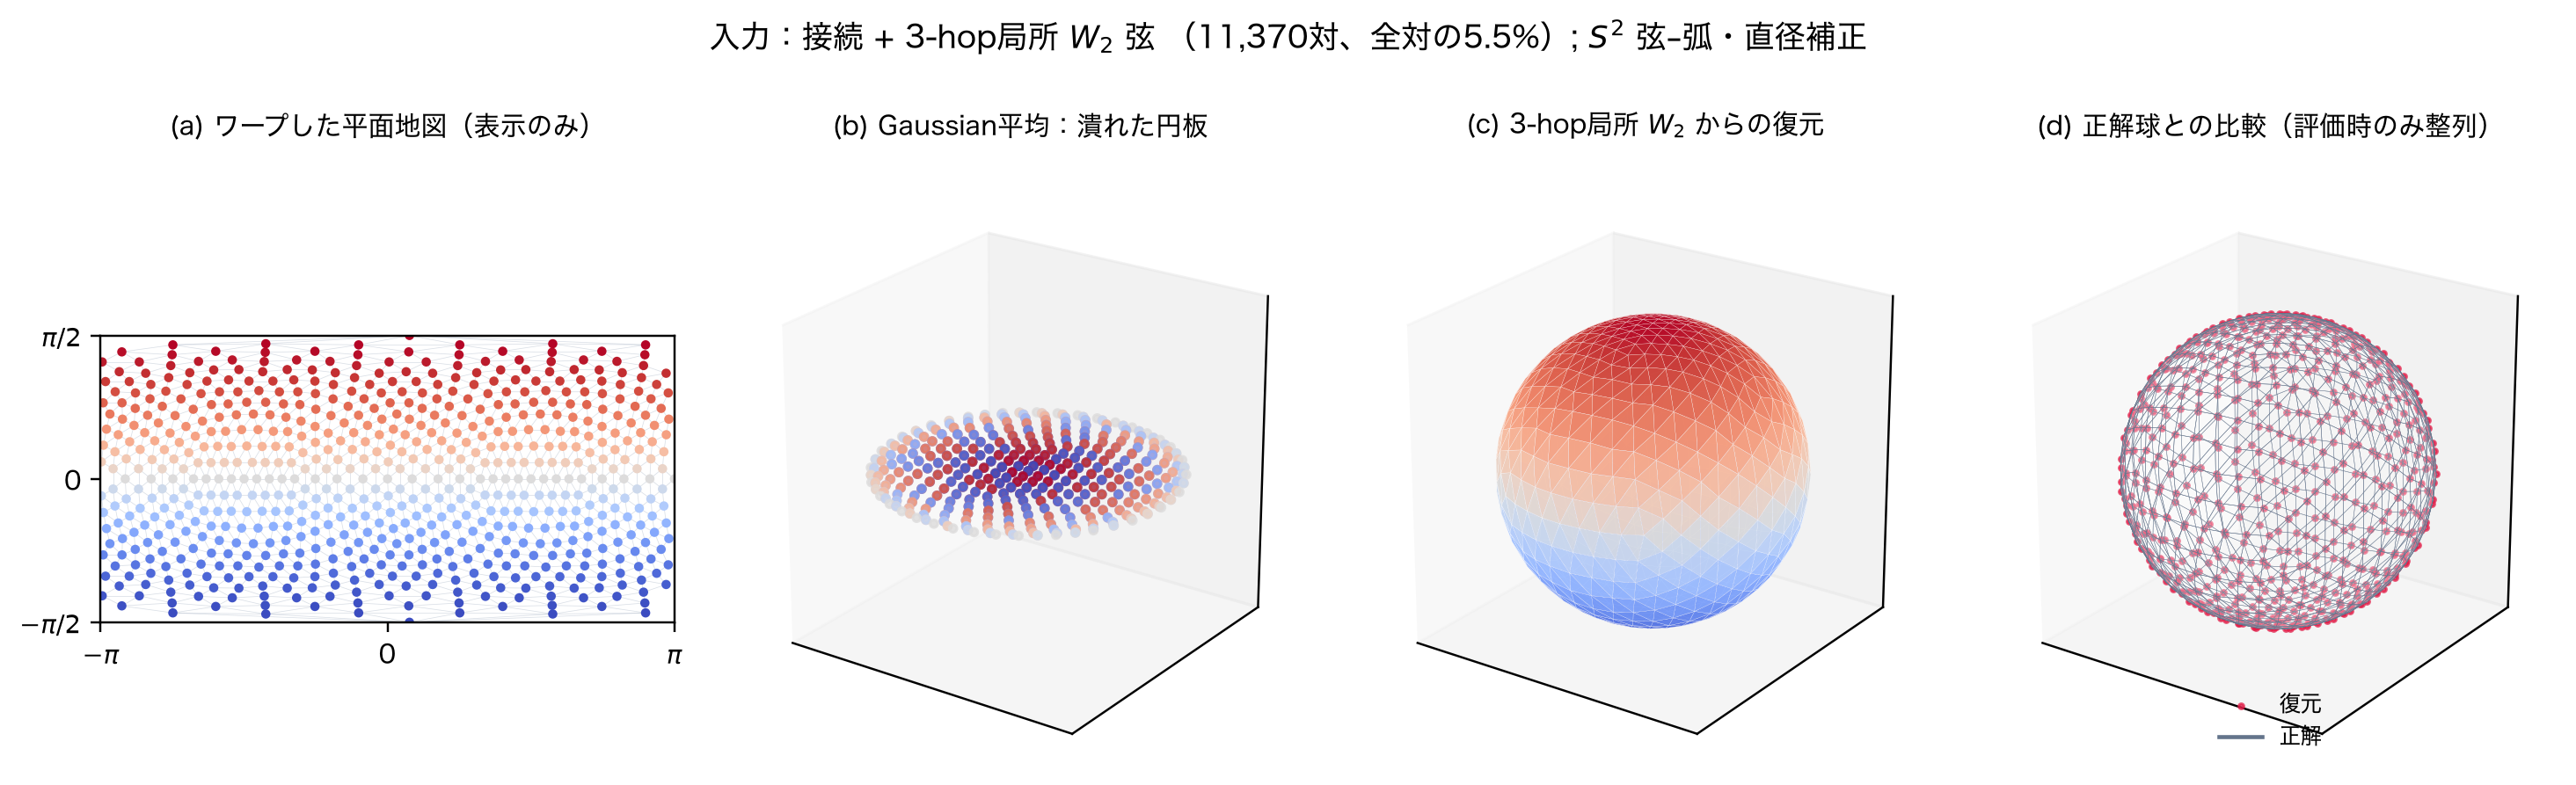
\includegraphics[width=0.99\textwidth]
 {experiments/wasserstein_surface_reconstruction_pipeline_ja.png}
 \caption{頂点数642、局所長さノイズ1\%における入出力。(a)は変形地図の表示であり、
 推定器への入力ではない。(b)のガウス平均は南北の情報を失う。定曲率推定器は、位相と
 全点対 $W_2$ 弦長のうちわずか5.53\%だけから(c)を出力する。(d)では、隠れた頂点を
 解答の位置合わせと重ね描きにだけ用いる。視覚的な結論は、まさに平面地図の比喩に対応する。
 局所移動時間から、失われた球面スケールが復元される。}
 \label{fig:wasserstein-surface-pipeline}
\end{figure*}

\subsection{結果}
\label{sec:surface-results}

\paragraph{OTは欠落した座標を保持する}
すべての試行で、一般ガウス $W_2$ 公式で計算した距離と隠れた3次元弦長の最大差は
$1.5\times10^{-15}$ 以下である。最細問合せグラフでは、共分散の最小固有値は $1.754$、
問合せ共分散対の $98.35\%$ は非可換である。さらに、生の共分散Frobenius差に対して一つの
大域スケールを正解から最適化しても、パラメータ距離の相対RMSEは $0.01245$ 残る一方、
Wasserstein恒等式は機械精度で成立する。平均のみのRMSEは $0.6538$ であり、平面円板では
正解対象を表現できない。図~\ref{fig:wasserstein-surface-pipeline} は、局所Wasserstein長が
欠落した次元を復元することを示す。

\paragraph{解像度とともに復元精度が向上する}
厳密観測では、相対測地距離誤差は、頂点数 $12,42,162,642$ に対して
\begin{equation}
 0.0985,\ 0.0392,\ 0.00915,\ 0.00261
 \label{eq:observed-distance-sequence}
\end{equation}
と減少する。位置合わせ後の3次元RMSEも同様に
\begin{equation}
 0.1365,\ 0.0400,\ 0.0105,\ 0.00287.
 \label{eq:observed-shape-sequence}
\end{equation}
と減少する。
最粗の12頂点メッシュでは、PL半径の過小推定により、ノイズなし問合せの $24.2\%$ で
弦長--弧長変換の引数がクリップされる。レベル1--3のノイズなし条件ではクリップはなく、
三つの細かい解像度点および最細メッシュの結論には影響しない。
頂点数642では、位相のみの対照は $0.1363$、通常MDSは $0.3616$、
平均円板は $0.6538$ にとどまる。したがって、結合関係と $S^2$ 出力制約だけでは
結果を説明できない。復元したクエリ弦長の相対ストレス（relative stress）は、
ノイズなしで $0.00330$ である。
残るグラフ近似誤差とスペクトル近似誤差を隠さず定量化している。対称Hausdorff誤差は、
厳密辺長で $0.00337$、ノイズ1\%で $0.00678$ である。

\begin{table*}[t]
\centering
\small
\caption{疎な3-hop局所Wasserstein弦長と定曲率 $S^2$ の弦--弧・直径補正による球面復元（最細メッシュ、平均 $\pm$ 標準偏差）。}
\label{tab:wasserstein-surface-reconstruction-ja}
\resizebox{0.98\textwidth}{!}{%
\begin{tabular}{@{}lccccccc@{}}
\toprule
ノイズ & 測地誤差 & 曲率RMSE（PL） & 非正欠損率 & 球面3D RMSE & 位相のみ & 通常MDS & 平均のみ \\
\midrule
0.0\% & 0.0026 $\pm$ 0.0000 & 0.000 $\pm$ 0.000 & 0.000 $\pm$ 0.000 & 0.0029 $\pm$ 0.0000 & 0.1363 $\pm$ 0.0000 & 0.3616 $\pm$ 0.0000 & 0.6538 $\pm$ 0.0000 \\
0.5\% & 0.0031 $\pm$ 0.0000 & 1.169 $\pm$ 0.067 & 0.202 $\pm$ 0.016 & 0.0031 $\pm$ 0.0000 & 0.1363 $\pm$ 0.0000 & 0.3621 $\pm$ 0.0002 & 0.6538 $\pm$ 0.0000 \\
1.0\% & 0.0044 $\pm$ 0.0001 & 2.324 $\pm$ 0.071 & 0.326 $\pm$ 0.007 & 0.0035 $\pm$ 0.0001 & 0.1363 $\pm$ 0.0000 & 0.3620 $\pm$ 0.0011 & 0.6538 $\pm$ 0.0000 \\
2.0\% & 0.0071 $\pm$ 0.0002 & 4.733 $\pm$ 0.175 & 0.415 $\pm$ 0.011 & 0.0052 $\pm$ 0.0003 & 0.1363 $\pm$ 0.0000 & 0.3610 $\pm$ 0.0015 & 0.6538 $\pm$ 0.0000 \\
\bottomrule
\end{tabular}
}%
\end{table*}


表~\ref{tab:wasserstein-surface-reconstruction-ja} が示すように、弦長ノイズ1\%でも、定曲率推定器の
測地距離誤差は $0.00437$、3次元RMSEは $0.00349$ にとどまる。ノイズ2\%では、それぞれ
$0.00706$ と $0.00518$ である。これらの小さな曲面誤差は、
第~\ref{sec:spherical-estimator}節の強い $S^2$ 射影を条件とする。任意のノイズ付き計量も
同様に容易に埋め込めることを示す証拠ではない。

\begin{figure*}[t]
 \centering
 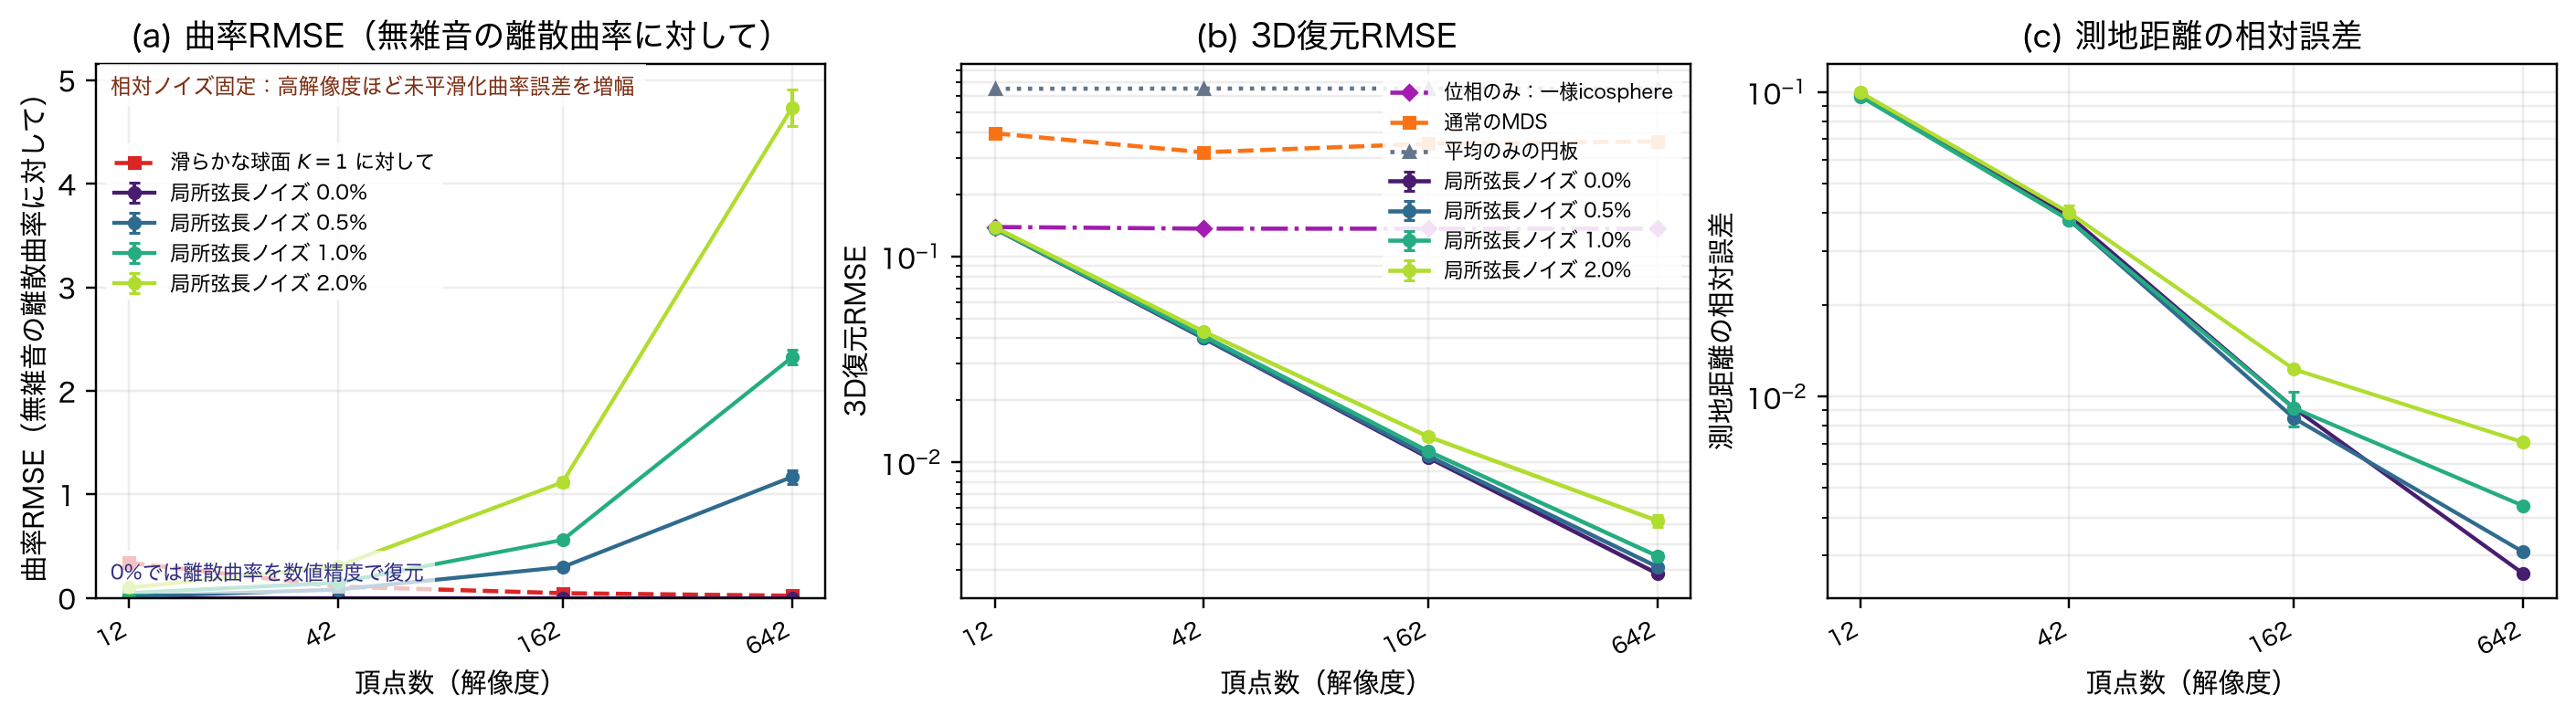
\includegraphics[width=0.625\textwidth]
 {experiments/wasserstein_surface_reconstruction_errors_ja.png}\hfill
 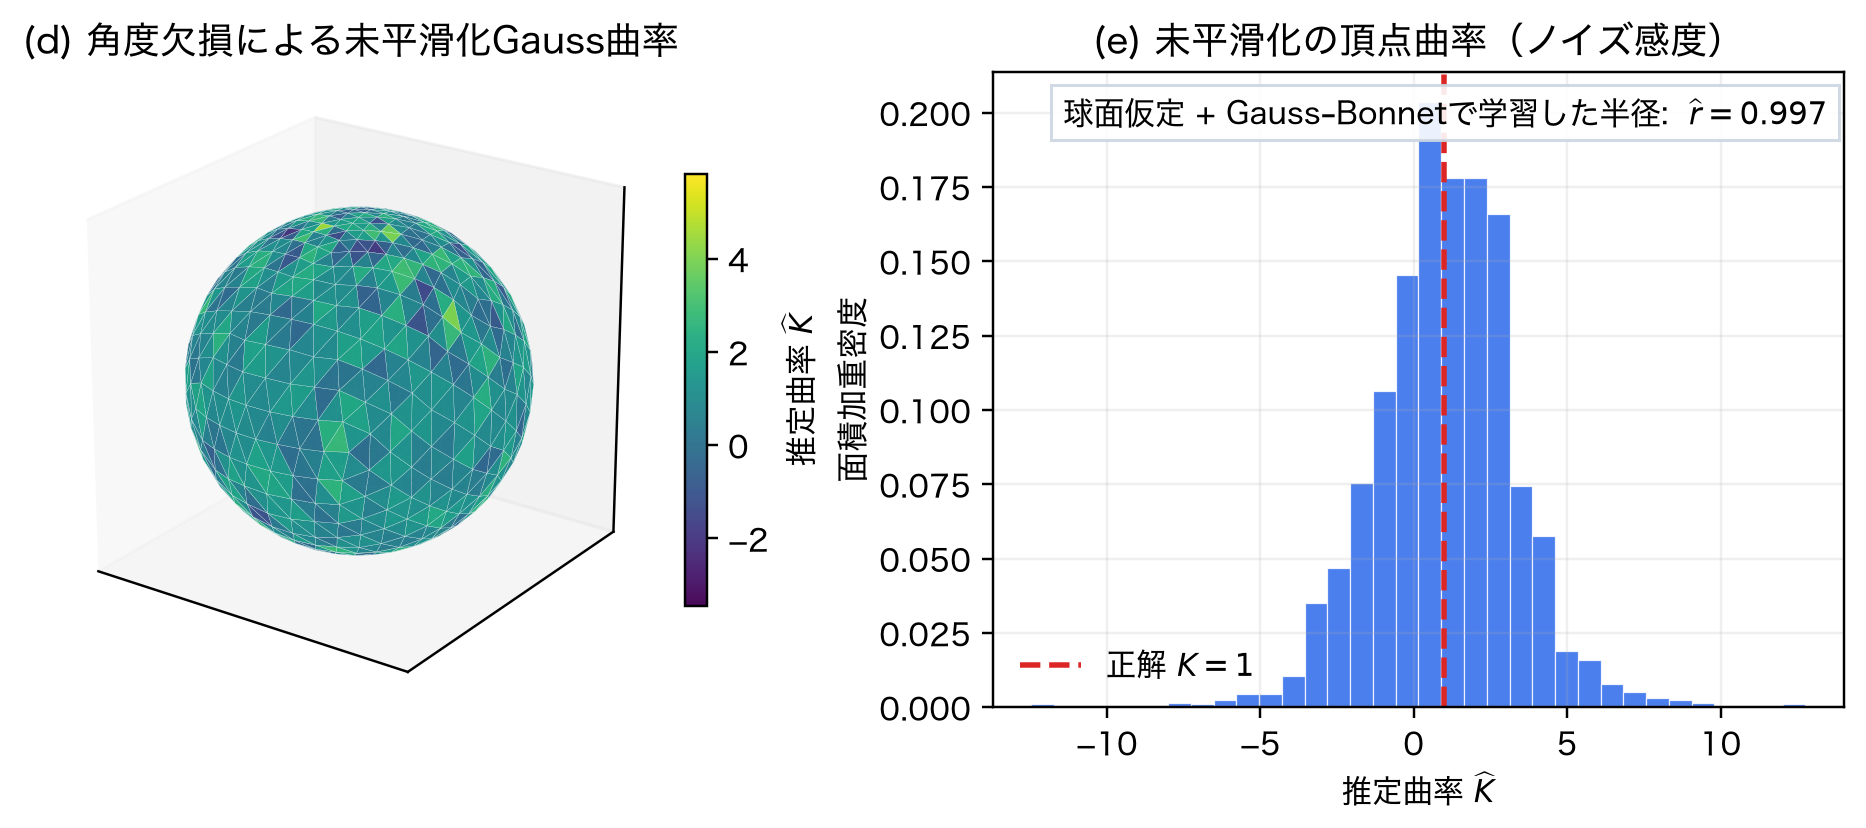
\includegraphics[width=0.355\textwidth]
 {experiments/wasserstein_surface_reconstruction_curvature_ja.png}
 \caption{解像度により、二つの統計的レジーム（regime）が分離される。(a)--(c)：固定した小さな
 相対ノイズのもとでも、大域距離と定曲率3次元復元は解像度とともに改善するが、生の
 面積正規化曲率はノイズを増幅する。(d)--(e)：頂点数642、ノイズ1\%で未平滑の曲率は
 広い分布をもち、学習半径が $0.997$ であっても負になりうる。これは
 式~\eqref{eq:noise-amplification} と定性的に整合する。大域的に良好な球面復元は、
 点ごとの曲率復元を意味しない。}
 \label{fig:wasserstein-surface-errors}
\end{figure*}

\begin{figure*}[t]
 \centering
 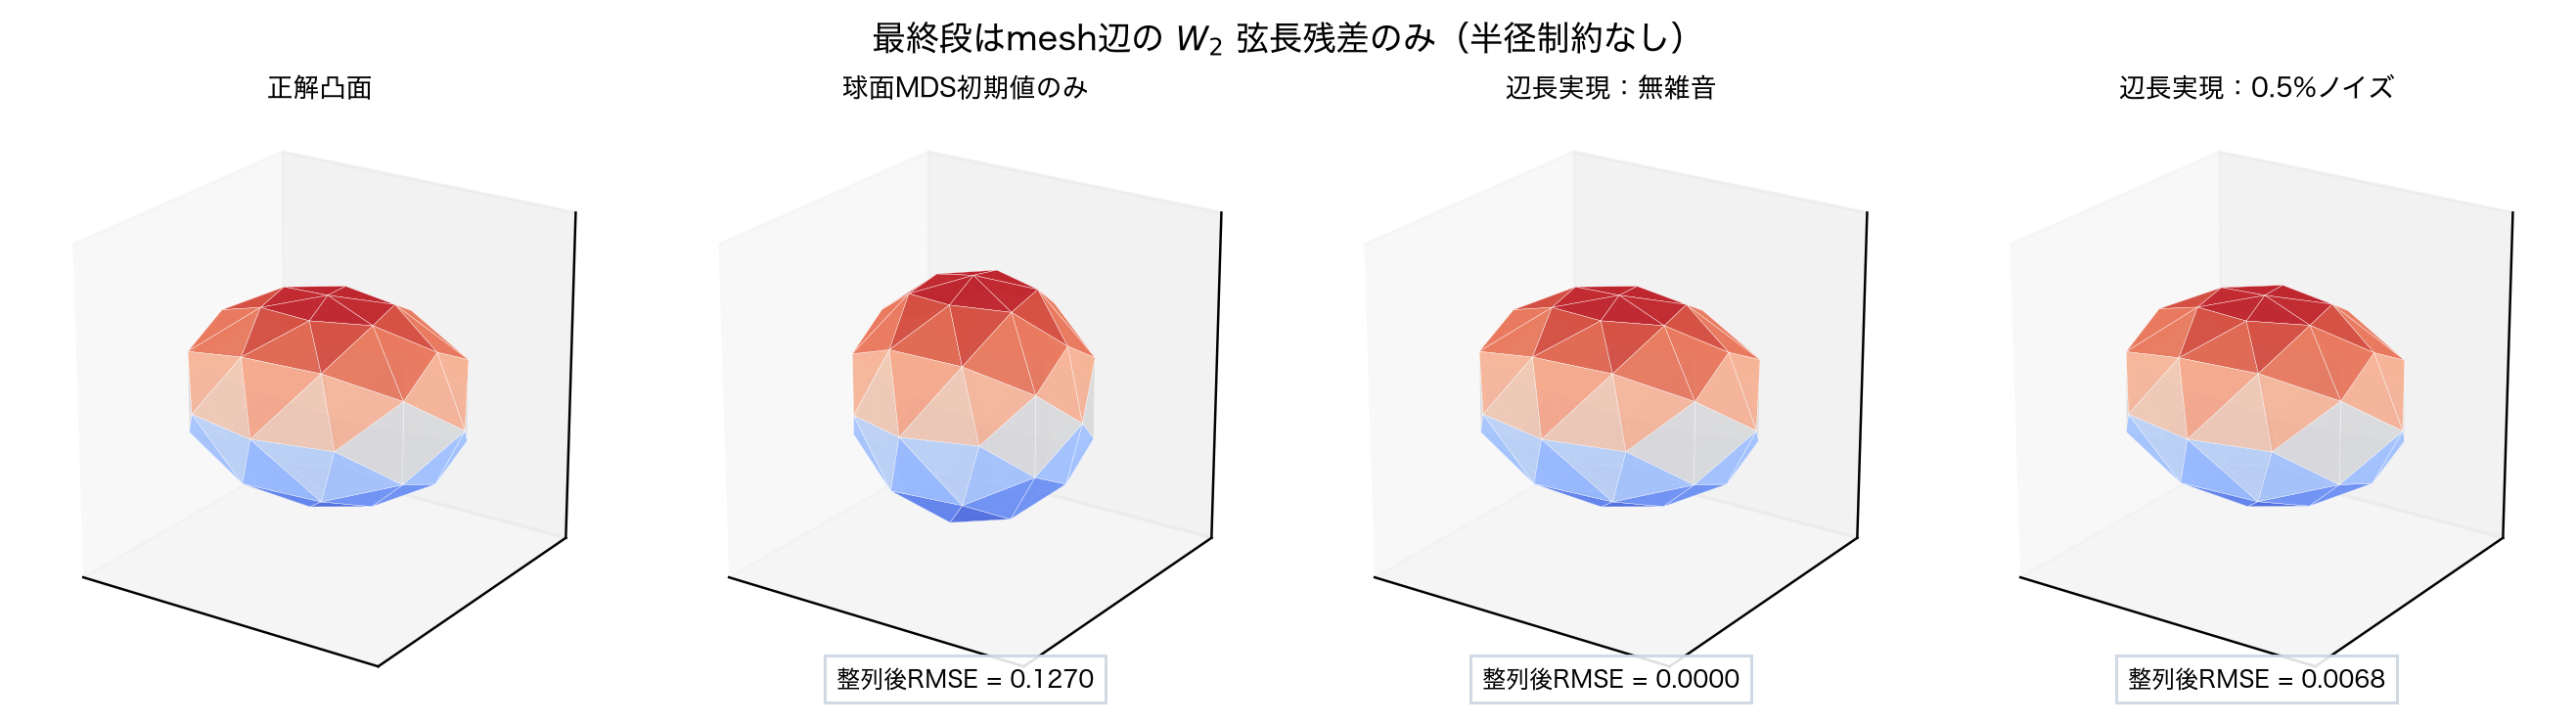
\includegraphics[width=0.98\textwidth]
 {experiments/convex_edge_realization_prototype_ja.png}
 \caption{非球形の楕円体状凸多面体に対する、辺長だけからの実現。列は隠れた正解、
 明らかに不正確な球面初期値、厳密辺長からの実現、0.5\%摂動辺長からの実現を示す。
 最終段階で用いるのはメッシュ辺上のWasserstein弦長残差だけである。表示したノイズ付き
 結果は乱数種0であり、球面・楕円体の全試行は表~\ref{tab:convex-edge-rigidity-ja} に示す。}
 \label{fig:convex-edge-realization}
\end{figure*}

\paragraph{点ごとの曲率が最も難しい}
厳密な長さでは、ノイズなしPL対象に対する曲率誤差は機械精度で0となる。頂点数642で残る
滑らかな $K=1$ に対するRMSE $0.0218$ は、離散化に由来する。固定相対ノイズの挙動は
異なる。同じ解像度で、長さノイズ $0.5\%,1\%,$ および $2\%$ は、生の離散曲率RMSE
$1.17,2.32,$ および $4.73$ をそれぞれ生じる。ノイズ1\%では、頂点の $32.6\%$ が
非正の角欠損をもつ。

これは、式~\eqref{eq:noise-amplification} における決定論的な区別と定性的に整合する。
同定理が用いるのは最大辺誤差である一方、\eqref{eq:multiplicative-noise} では独立な
対数正規誤差（log-normal errors）を生成する。小さな $\sigma$ に対し、有限な問合せ辺集合
における相対誤差の最大絶対値は、典型的には $\sigma\sqrt{\log|E_{\mathrm q}|}$ オーダーである。
したがって、このスイープが検証するのは予測された増幅パターンであり、定理の定数ではない。
$\varepsilon\asymp\eta h$ なら、角欠損誤差は $O(\eta)$ だが、頂点面積で除すことにより
曲率密度誤差は $O(\eta/h^2)$ となる。したがって、固定相対ノイズのもとでの細分化は、
大域距離の復元を改善する一方、未平滑な点ごとの微分量を悪化させる。細かいスケールで
整合的な曲率を得るには、ノイズを小さくするか、正則化された推定器が必要である。
特に、正の角欠損条件~\eqref{eq:convexity-noise} は、ノイズを加えた最細メッシュの試行では
成立しない。そこで良好な球面出力が得られるのは、明示した定曲率射影によるものであり、
凸実現定理を適用した結果ではない。

\subsection{標準球面を越える同一骨格復元}
\label{sec:convex-realization-experiment}

球面に対する一連の実験は視覚的に単純だが、命題~\ref{prop:rigidity} の一般的な実現過程を
実行してはいない。そこで、小規模かつ独立した距離幾何（distance geometry）実験を追加する。
推定器が受け取るのは
$(|V|,F,E,\{\widehat\ell_e\}_{e\in E})$ だけである。球面多次元尺度構成法
（spherical MDS）から凸な初期分枝を得た後、継続法（continuation）により
\begin{equation}
 \sum_{(i,j)\in E}
 \left(
 \frac{\norm{X_i-X_j}-\widehat\ell_{ij}}
 {\overline\ell}
 \right)^2 .
 \label{eq:edge-realization-objective}
\end{equation}
を最小化する。ここで $\overline\ell$ は、観測された辺長の平均である。
観測された三辺長から一つの非退化なアンカー三角形を配置し、ユークリッド
運動のゲージ自由度を除く。局所凸性ペナルティを用いるのは41段階の継続過程だけである。
最後の最小二乗による精密化には、117個の自由座標と117個の非アンカー辺残差があり、半径、
行の正規化、球面損失、正解座標はいずれも含まれない。

球面上の42標本点の凸包と、それらを軸長 $(1.20,1.00,0.80)$ で線形変換した点の凸包を試す。
後者は、非定数ガウス曲率をもつ滑らかな狭義凸曲面を標本化した、楕円体状凸多面体である。
隠れたガウス構成では、引き続き
$W_2(\mu_x,\mu_y)=\norm{x-y}$ が成り立つ。厳密弦長に対する位置合わせ後RMSEは、球面で
$3.25\times10^{-15}$、楕円体で $2.17\times10^{-15}$ である。一方、楕円体に対する
球面初期値のRMSEは $0.1270$ である。3乱数種の平均RMSEは、辺ノイズ0.5\%で
$0.00601$ と $0.00720$、1\%で $0.01094$ と $0.01463$ である。14個の出力はすべて、
凸包に42頂点をすべて保持し、面数もちょうど指定した80となる。

\begin{table}[t]
\centering
\small
\caption{ノイズ下の同一骨格剛性監査。Frobenius誤差は最適な $E(3)$ 整列後、上界は $2\|\Delta\ell\|_2/s_X$、比は誤差/上界である。数値は平均 $\pm$ 標準偏差、Hullは全頂点・facet一致数を表す。}
\label{tab:convex-edge-rigidity-ja}
\resizebox{\linewidth}{!}{%
\begin{tabular}{@{}lccccc@{}}
\toprule
条件 & $\|\Delta\ell\|_2$ & $\|\widehat X-X\|_F$ & 局所上界 & 比 & Hull \\
\midrule
球面 0.5\% & 0.0308 $\pm$ 0.0014 & 0.039 $\pm$ 0.0011 & 0.175 $\pm$ 0.0077 & 0.222 $\pm$ 0.0047 & 3/3 \\
球面 1.0\% & 0.0589 $\pm$ 0.0028 & 0.0709 $\pm$ 0.0041 & 0.335 $\pm$ 0.016 & 0.212 $\pm$ 0.01 & 3/3 \\
楕円体 0.5\% & 0.0328 $\pm$ 0.0038 & 0.0467 $\pm$ 0.0067 & 0.229 $\pm$ 0.026 & 0.203 $\pm$ 0.0057 & 3/3 \\
楕円体 1.0\% & 0.0638 $\pm$ 0.0078 & 0.0948 $\pm$ 0.018 & 0.445 $\pm$ 0.054 & 0.211 $\pm$ 0.02 & 3/3 \\
\bottomrule
\end{tabular}%
}
\end{table}


ノイズを含む場合に辺長へ厳密に適合させることは、ノイズ除去ではない。球面三角形分割では
$|E|=3|V|-6$ であり、局所剛性により、十分小さく摂動された長さベクトルは、一般には異なる
近傍の凸多面体へ写される。観測された座標誤差は、命題~\ref{prop:rigidity} の安定性量である。
報告したRMSEは、その $|V|^{-1/2}$ 正規化である。正解での剛性行列は階数
$120=3|V|-6$ をもち、$s_X$ は球面で $0.352$、楕円体で $0.287$ である。12個の
ノイズ付き試行はすべて局所スケール $2\norm{\widehat\ell-\ell}_2/s_X$ を下回り、
誤差と上界の比の最大値は $0.233$ だった。このプロトタイプは対象とする局所分枝を
数値的に検証するが、継続法の大域収束を証明するものではない。

\section{適用範囲と結論}
\label{sec:limitations}

制御実験から、正確かつ視覚的に検証可能な次の結論が得られる。局所Wasserstein弦長が
隠れた標準球面計量（round metric）を符号化する確率的デコーダーでは、疎なクエリから、
デコーダーの微分を用いずに大域移動時間と球面を復元できる。理論はこれとは別に、一般の
同一骨格狭義凸
多面体について辺長から何が決まるかを述べ、式~\eqref{eq:end-to-end-sphere} により
球面に対するエンドツーエンド（end-to-end）誤差分解を与える。この分解が対象とするのは
近傍の同一骨格凸実現であり、実装したグラフ最短路・球面尺度構成パイプラインそのものの
保証ではない。

いくつかの仮定は明示的に残る。位相と三角形分割は入力として与える。球面に対する一連の
実験は、定曲率、既知の対蹠点被覆、および厳密な $W_2$ をもつガウスベンチマークを
仮定し、その全点対数値計算段階は $O(|V|^2)$ のメモリを用いる。辺長だけを用いる実験は
42頂点かつ各ノイズ条件3乱数種に限られ、継続法が正しい凸分枝にとどまることを必要とし、
大域収束を保証しない。
いずれの実験もMNISTの真の幾何を推定せず、曲率を平滑化せず、ミニマックス（minimax）
統計率も与えない。学習デコーダーではさらに、有限標本誤差と数値OT誤差が生じる。
これらは理論の辺誤差項に入るが、本実験では評価しない。

したがって、ヤコビ行列に基づく潜在幾何からの概念的変更は単純である。幾何を、観測可能な
局所分布距離からの逆問題として扱える。制御された場合、答えは単なる曲率ヒートマップでは
ない。Wasserstein観測誤差と有限メッシュ近似誤差に分解可能な誤差をもつ、復元曲面そのもので
ある。
